%
\documentclass[11pt]{article}
\usepackage[a4paper, margin=1in
]{geometry}
\usepackage{graphicx}
\usepackage{xcolor}
\usepackage{kpfonts}
\usepackage{fancyhdr}
\usepackage[
  style=ieee,
]{biblatex}
% use package for referencing figures
\usepackage{caption}
\usepackage{subcaption}
\usepackage[capitalise]{cleveref}

\usepackage[skip=1em]{parskip}

\pagestyle{fancy}

\title{\vspace{-2em}\small{Analysis of Week 12's Paper}\\\LARGE{Chromosal Organization through Loop Extrusion}\vspace{-1em}}
\author{Minghang Li}
\date{\vspace{-1em}}

\fancyhf{}
\lhead{Current Topics in Biophysics}
\rhead{\today}

\cfoot{\thepage}

\setlength{\parindent}{0ex}

\bibliography{report}

% -- end preamble --

\begin{document}

\maketitle \thispagestyle{fancy}

\bigskip
\hrule \vspace{1pt}
\hrule height 1pt
\bigskip

% the most important part it to explain

%  + what the general question is that is being addressed. that will include some general context on chromosome conformations and chromatin accessibility. (DONE!)
%  + how we learn about chromatin conformations (Hi-C etc) (DONE!)
%  + a discussion of the author's approach, the model, and the results.
%  * what the strength and weaknesses of the model are, what is left unexplained
%  * What could be done next? What has been done since?

% This discussion will include answers to many of the questions we discussed. You'll usually include some figures from the paper to make your point.

\begin{abstract}
  \noindent Week 12's lecture discussed the paper by Fudenberg et. al., titled by "\textit{Formation of Chromosomal Domains by Loop Extrusion}". It investigated the underlying mechanism of the formation of one of the most common and important chromosomal structure -- Topologically Associating Domains (TADs). It proposed the hypothesis that TADs are formed by loop extrusion regulated by Boundary Elements (BEs) and Loop Elongation Factors (LEFs) and tested the hypothesis through rigorous modelling and simulation.
\end{abstract}

\section{Background Introduction}

\subsection{Chromosomal Conformation Capture (3C) Technologies}

The genetic information stored in DNA sequences is not presented in a linear manner, but is rather folded and organized into three-dimensional (3D) structures, thereby allowing remotely located genomic elements interact with each other. To understand the 3D spatial genome organization better, various techniques have been developed over the years. Beyond the conventional microscopy observation that uncovered some basic principles about genome microscopy, the development of chromosome conformation capture (3C) technologies has also produced many important insights into the chromatin structure \cite{denker_second_2016}.

The 3C technology was first introduced in 2002 by Dekker et. al. originally in the hope of studying the folding of yeast chromosome \cite{dekker_capturing_2002}. It quickly inspired the emergence of an abundance of 3C-derived genomics methods. \cref{fig:3C} shows an overview of the 3C-derived technologies, which all start with the same steps. First, the DNA is crosslinked using a fixative agent, most often formaldehyde, to preserve the 3D representation of the genome. Second, the crosslinked DNA is digested with restriction enzymes to generate DNA fragments of a certain size. The DNA fragments are then ligated to specific adapters and amplified by PCR. The amplified DNA fragments are then sequenced and the sequence information is used to infer the spatial relationship between the captured DNA fragments \cite{wit_decade_2012}. Amongst all the 3C-derived technologies, Hi-C is probably the most widely used one. In Hi-C, the restriction ends of DNA fragments are filled in with biotin labeled nucleotides before the ligation step. Following a blunt ligation (usually by T4 DNA ligase), the biotin-labeled DNA fragments are purified and then captured by streptavidin-coated magnetic beads. After biotin-pulldown, the fragments are sheared into reads and then mapped back to the reference genome to generate a contact map, which is then used to score and infer the 3D structure of the genome \cite{wit_decade_2012}. Biotin pull-down and paired-end sequencing enables the detection of ligation junctions, and Next Generation Sequencing (NGS) methods makes such "all versus all" detection at a genome-wide scale possible.

% insert figure 1
\begin{figure}[htbp]
  \centering
  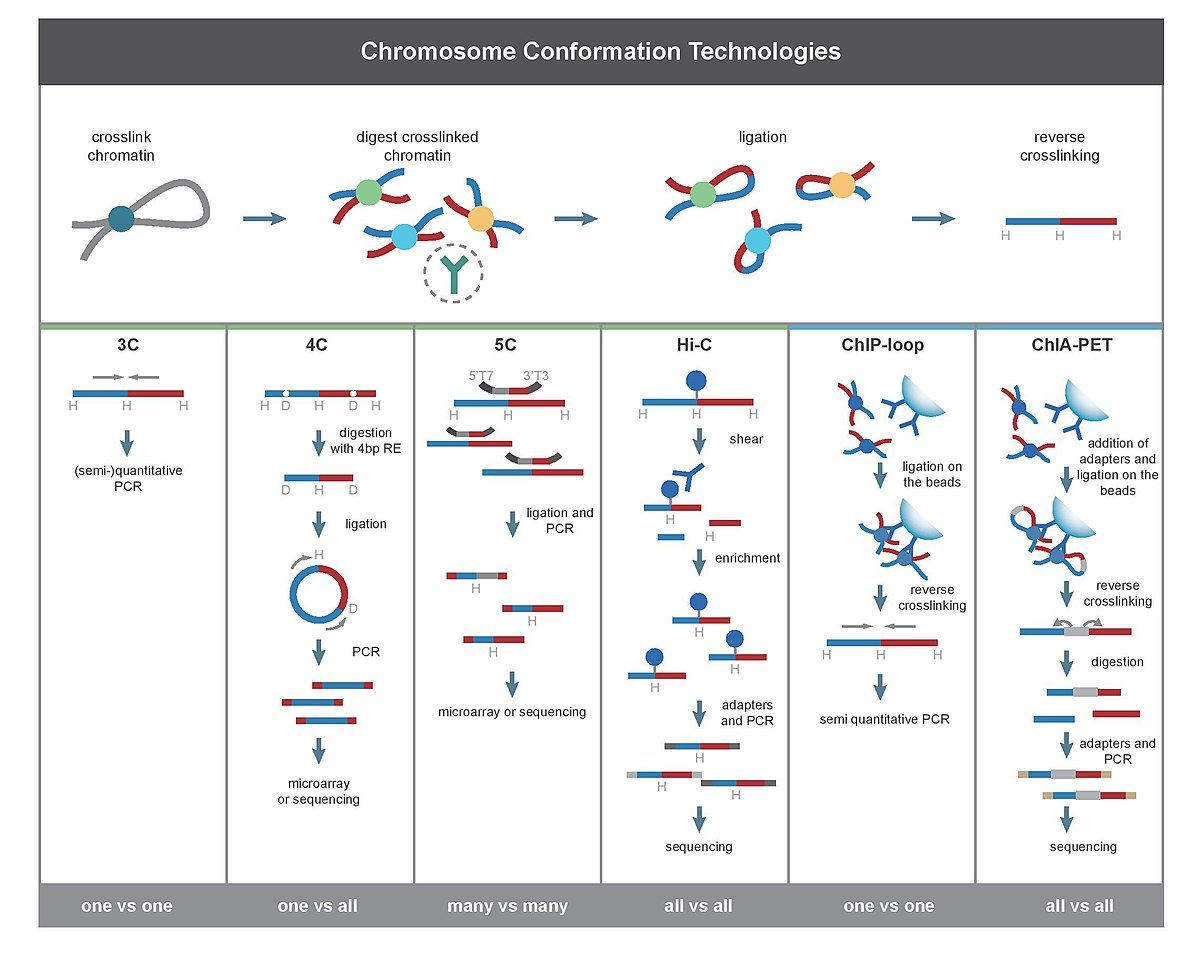
\includegraphics[width=0.8\textwidth]{assets/20221212064821.png}
  \caption{\textbf{An Overview of the 3C Technologies.}This figure comes from \cite{li_chromatin_2014}, which was adapted from \cite{wit_decade_2012}}
  \label{fig:3C}
\end{figure}

\subsection{Two Major Classes of Chromosomal Patterns}

Hi-C is capable of capturing the 3D structure of the genome at a resolution of kb level. In the Hi-C contact maps, two major classes of patterns are most evident. The first one is the A/B compartmentalization which shows checkerboard-like patterns \cite{mirny_two_2019}. The A compartment is usually gene-rich, transcriptionally active and accessible (characterized by DNase I sensitivity), and the B compartment is usually the heterochromatin region that is low in expression and has repressive histone marks \cite{denker_second_2016}\cite{wit_decade_2012}. The second one is the Topologically Associating Domains (TADs) which are characterized as continuous regions of mildly (2-4 folds) higher contact frequency than between loci in neighboring TADs \cite{mirny_two_2019}. They usually reside within a single contiguous compartment and don't necessarily exhibit the characteristic "checkerboard" pattern as A/B compartment does \cite{fudenberg_formation_2016}. 50\% of TADs have peaks of interactions at their boundaries, and they are capable of forming dynamic boundaries \cite{rao_3d_2014}. Up until the publishing of this paper, the formation of TADs was still not well understood. Previous works have proposed TADs forming mechanism based on similar monomer attraction \cite{jost_modeling_2014} and supercoiling \cite{benedetti_models_2014}, yet they fail to explain the formation of TADs in a satisfactory manner.

% insert figure 2
\begin{figure}[htbp]
  \centering
  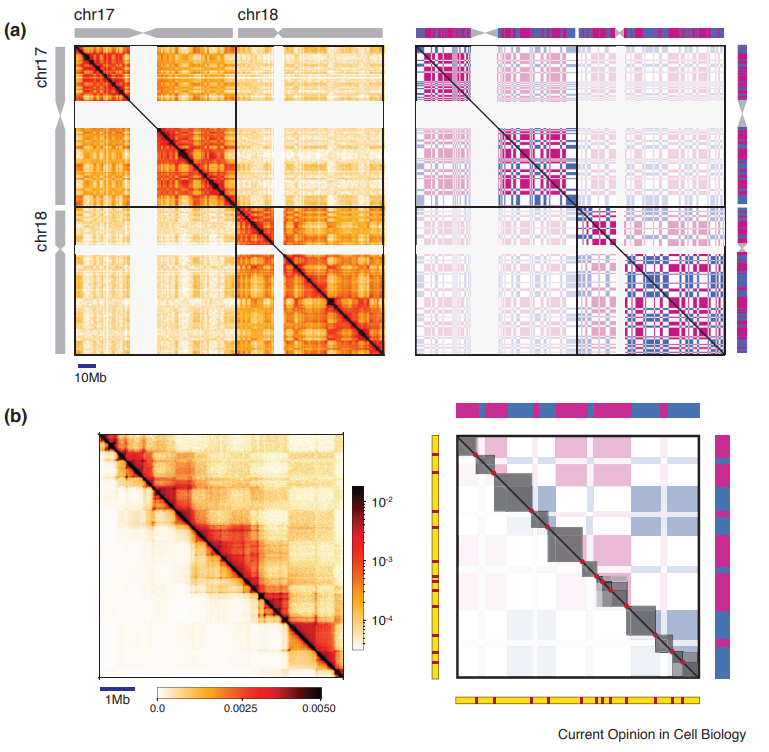
\includegraphics[width=0.8\textwidth]{assets/Snipaste_2023-01-13_15-53-18.png}
  \caption{\textbf{Hallmark Patterns in Hi-C Maps: Compartmentalization and TADs.} This figure comes from \cite{mirny_two_2019}. Fig (a) shows the A/B compartmentalization pattern, and Fig (b) shows the TADs pattern.}
  \label{fig:TAD}
\end{figure}

\section{Brief Summary of the Model}

To give out a satisfactory explanation for TAD formation, the authors proposed a loop-extrusion based mechanism. In this process, TADs are formed through the dynamic introduction of chromatin loop by \textit{cis}-acting loop-extruding factors (LEFs) and are bounded by boundary elements (BEs). The loop extrusion process was modelled by coupling the 1D dynamics of LEFs with 3D polymer dynamics. The following subsections will give a concise summary of the details of the proposed mechanism.

\subsection{Basic Settings of the 1-D Model}

The authors first defined the dynamics of LEFs with BEs. The translocation of LEFs along the chromatin fiber was simulated on a 1D lattice, where each position was characterized by association (birth) probability, dissociation (death) probability and BE occupancy (stalling probability). The LEF molecule was modelled by "two heads" connected with a linker, analogous to SMC protein complexes. Each head of the LEF occupied one lattice position and cannot be overlapped except for at birth events. At each time-step, each LEF head translocates to the neighboring lattics position in opposite direction until encountering another LEF head or a boundary element (BE). The stalling of one LEF head does not affect the translocation of the other LEF head.
At each discrete unit of time, a LEF undergoes dissociation with a probability that is equal to the maximum value of the death probability. For the occurrence of birth events, the two heads of the LEF are either initiated on the same lattice location or on neighboring sites (when the site immediately to the right of the selected site is unoccupied) with a probability of 0.5. The dynamics of LEFs were depicted in \cref{fig:LEF dynamics}.

% insert figure 3
\begin{figure}[htbp]
  \centering
  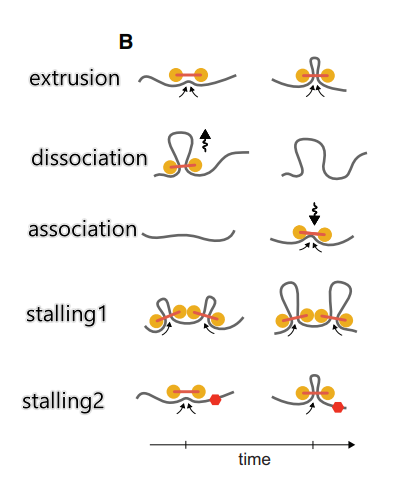
\includegraphics[width=0.5\textwidth]{assets/image-20221212095109951.png}
  \caption{\textbf{The Dynamics of LEFs.} This figure comes from \cite{fudenberg_formation_2016}.}
  \label{fig:LEF dynamics}
\end{figure}

\subsection{Basic Settings of the 3-D Polymer Model}

As is later shown in the paper, the 1-D model can very well depict the TAD as an average of experiments from many cells, yet it is difficult to model insulation solely by the 1-D model. For example, an enhancer and promoter separated by 100kb can still come in contact in the 3D space. To account for this, the authors proposed a 3D polymer model to simulate the 3D structure of the chromatin fiber.

The 3D chromatin model is a polymer connected by 10-nm monomers (roughly the size of 3 nucleosomes or 600bp) subject to Langevin dynamics, which according to my understanding models the stochastic behavior of molecules in solvent. The monomers are further modelled by excluded volume interactions, which prohibits monomer overlapping, and are linked with harmonic bonds that restrict their relative position but allow for rotation in certain degrees (stiffness) and chain passing (which represents the activity of topoisomerase and enables loop twisting and loop inside loops).

\subsection{Connecting the 1-D and 3-D Models}

LEFs serve as the connection points between 1-D and 3-D models: they affects the monomers of the 3-D model by introducing additional harmonic bond between the monomers held by the two heads of the LEFs. The bond is constantly reassigned to increasingly separated pairs of monomers as the LEF heads move along the chromosome. Furthermore, before starting the 3D simulation, the 1D LEF dynamics was first run for 4 million steps to achieve convergence of LEF initial positions. At each 1-D simulation time step, according to the hyperparameter \textit{3D-to-1D dynamics}, the corresponding 3D Langevin dynamics simulations were performed before starting the 1D-simulation time steps.

\subsection{Important Parameters of the Model As A Whole}

To simplify the simulation effort and to account for the still-unknown biological setup of exact LEF dynamics parameters, the authors chose to first use a simple setting with uniform birth probability, constant death probability, a fix number of LEFs and a discrete nubmer of impermeable BEs. The parameters have been relaxed in latter explorations such as the permeability of BEs, or even different types of BEs. Under such scenario, the LEF dynamics can be well described by only two metrics: the LEF processivity ($\frac{2}{\text{death rate}}$) and LEF separation ($\frac{\text{total number of lattice sites}}{\text{number of LEFs}}$). The processivity accounts for the average size of the loop extruded by an LEF if not stopped early; and the separation represents the distance between two pairs of LEFs on average.

In the simulations, the authors tested various combinations of processivity and separation and analyzed the effects of these parameters on the shape of the TADs.

\section{Brief Summary of the Results}

\subsection{Evaluation of the Model}

The authors used a measurement called $P(s)$ (a function of genomic distance $s$) to test the ability of the model to reproduce Hi-C contact map data. They plotted $s-P(s)$ curves for the model and the experimental data they obtained and confirmed that the shapes are similar. To measure the reproduction quantitatively, they also determined the \textit{goodness of fit} using the geometric standard deviation of the ratios of the experimental data nad simulated $P(s)$ curves. Using such measures, the authors identified the best parameter settings (processivity and separation) to reproduce the experimental data.

% insert figure 4
\begin{figure}[htbp]
  \centering
  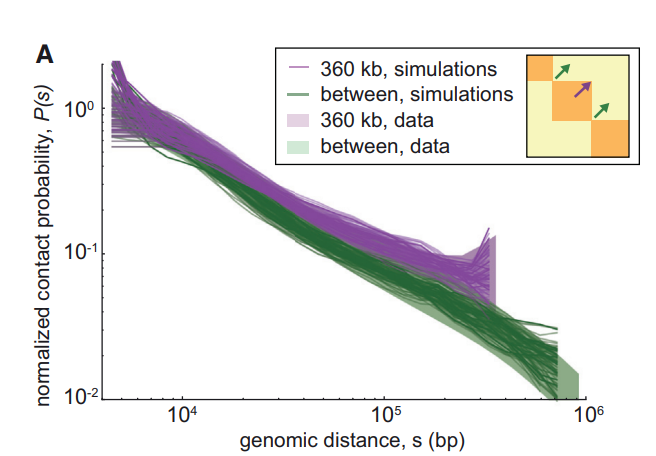
\includegraphics[width=0.8\textwidth]{assets/Snipaste_2023-01-13_17-49-12.png}
  \caption{\textbf{Evaluation of Model.} This figure comes from \cite{fudenberg_formation_2016}.  Experimental $P(s)$ (shaded areas) versus simulated $P(s)$ for the 100 best fitting parameter sets (lines, one per parameter set) within TADs (purple) and between
  TADs (green).}
  \label{fig: evaluation of model}
\end{figure}

\subsection{Proposed Candidates for BEs and LEFs}

It is natural to look for the possible molecular candidates for LEFs and BEs after building a successive model. As is summarized by the authors in the paper, it is highly likely that cohesin is a possible LEF in interphase. Cohesin is a Strutural Maintenance of Chromosomes (SMC) complex that have been proposed to be able to extrude loops of chromatin fiber and recently been proved to be able to move along the chromatin. They are also observed to be enriched at TAD boundaries and corner peaks, and removal of cohesin leads to the loss of TADs.

CCCTC-binding factor (CTCF) is a possible candidate for BEs. Similar to cohesin, CTCFs are also enriched at TAD boundaries and corner peaks, and the depletion of CTCF sleas to similar effect as cohesin depletion. Furthermore, CTCF is known to be able to interact with cohesin, especially in an orientation-dependent manner. More interestingly, inward-oriented CTCF sites are observed to occur at high frequency at TAD boundaries and corner-peaks, which is consistent with the model that CTCF is a BE.

\subsection{The Effect of Processivity and Separation}

As is shown in \cref{fig:processivity and separation}, the authors evaluated for the best parameters for the model as well as exploring the effect of changing the processivity and separation. The best agreement with Hi-C data is achieved for processivity of 120-240 kb and separation of 120 kb. It also shows that processivity affects the strength of the corner peak, while separation affects the strength of the TAD cliques as well as width of the TAD. The effect of processivity is especially natural since the larger the LEF processivity, the higher the probability of two LEFs to reach the BEs, hence the higher contact probability of the fragments at the end of TADs, resulting in the stronger corner peaks.

% insert figure 5
\begin{figure}[htbp]
  \centering
  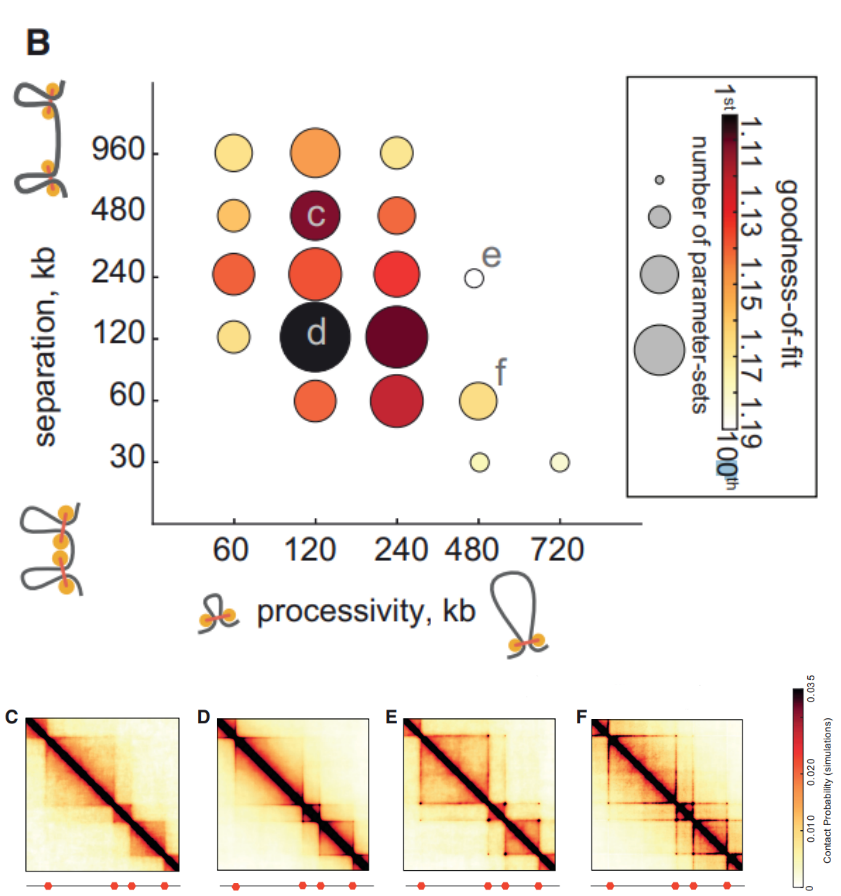
\includegraphics[width=0.6\textwidth]{assets/Snipaste_2023-01-13_18-19-27.png}
  \caption{\textbf{The Effect of Processivity and Separation.} This figure comes from \cite{fudenberg_formation_2016}. Figure C, D, E, F corresponds to the parameter set c, d, e, f in figure B, respectively.}
  \label{fig:processivity and separation}
\end{figure}

\subsection{Exploration of Alternative Hypotheses}

As is mentioned in the introduction, there are several other plausible hypotheses of interest. To prove the superiority and generality of the model, the authors investigated a few of alternative hypotheses and showed that they more or less failed to faithfully reproduce TADs in the simulation.

\subsubsection*{Investigate TAD formation Via Single Stable Loop}

As is shown in \cref{fig:Investigate TAD formation Via Single Stable Loop}, it is clearly shown that single stable loops are incapable of producing TADs. Conspicuously, the single table loops produce exceedingly strong corner peaks and no intermediate interactions that gives the characteristic cliques in the Hi-C contact map.

% insert figure 6
\begin{figure}[htbp]
  \centering
  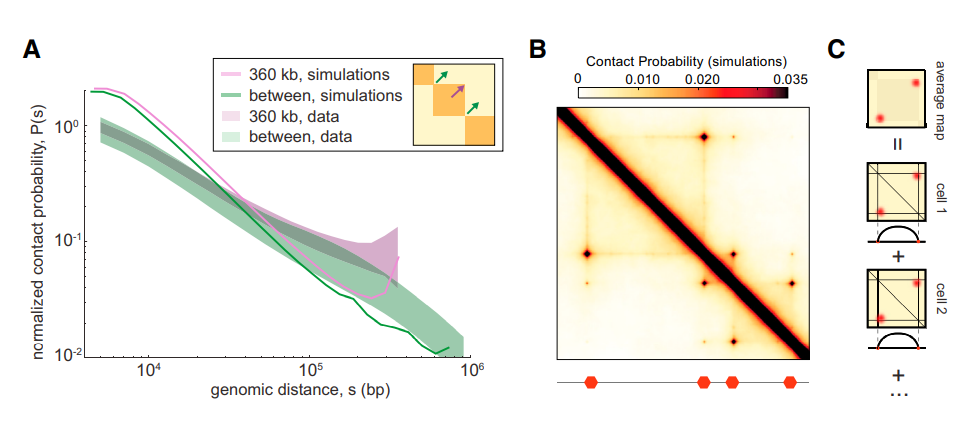
\includegraphics[width=0.8\textwidth]{assets/Snipaste_2023-01-13_18-37-34.png}
  \caption{\textbf{Investigate TAD formation Via Single Stable Loop.} This figure is exactly Figure 4 in \cite{fudenberg_formation_2016}. It shows that single stable loops are incapable of producing TADs.}
  \label{fig:Investigate TAD formation Via Single Stable Loop}
\end{figure}

\subsubsection*{Investigate TAD formation Via Solely Boundary Element Dynamics}

The model proposed by the authors do not rely on the direct physical blockade of LEFs by BEs to enable insulation between TADs, instead, it relies on the BEs to regulate the translocation of LEFs. However, it is possible that direct physical insulation of BEs can lead to the formation of TADs. To rule out the possibility that TADs simply result from the existence of bulky objects at boundaries, the authors tested such hypothesis in the simulation. They also investigated the effect of placing stiff chromatin fiber at BE location, which has similar effect as bulky BEs. The dimerization of BEs can also potentially lead to the formation of TADs -- this represents the scenario that proteins are capable of selectively bind specific genomic elements.

As is shown in \cref{fig:Investigate TAD formation Via Solely Boundary Element Dynamics}, it is very obvious that no TADs are formed at all when BEs are modelled by either bulky objects or stiff chromatin fibers. The direct BE-to-BE mechanism, despite showing some interaction between distal loci, cannot distinguish between chromosomal regions, and result in uniform peaks of contact probability accross all the BE pairs. It also have zero separating effect between TADs, resulting in no characteristic clique shape of TADs at all.

% insert figure 7
\begin{figure}[htbp]
  \centering
  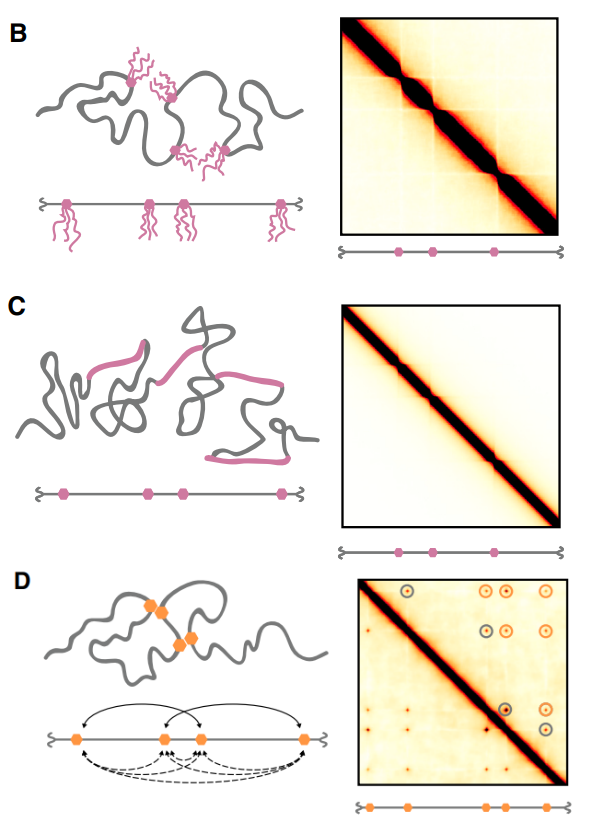
\includegraphics[width=0.6\textwidth]{assets/Snipaste_2023-01-13_18-53-59.png}
  \caption{\textbf{Investigate TAD formation Via Solely Boundary Element Dynamics.} This figure is part of Figure 5 in \cite{fudenberg_formation_2016}. Fig B models BE as bulky objects, Fig C models BE as stiff chromatin fibers, Fig D models the BE-to-BE TAD formation mechanism.}
  \label{fig:Investigate TAD formation Via Solely Boundary Element Dynamics}
\end{figure}

The simulation of the alternative hypotheses stress on the importance of the \textit{cis}-acting manner of LEFs along the chromatin as well as sophisticated interaction between BEs and LEFs.

\subsection{Exploration of Boundary Elements Properties}

It has been shown in literature that flipping solely the orientation of BEs (to be exact, the proposed molecular BE candidate, CTCFs) can lead to the merging of two TADs.

The authors analyzed cohesin ChIP-seq peaks and found that CTCFs were enriched in exact orientation dependent manner around strongly bound CTCF peaks, suggesting CTCF indeed acts as a BE that impedes loop extrusion in an orientation-dependent manner -- at strong CTCF binding sites, cohesins are enriched only in one direction but not the other. In weak CTCF binding sites, cohesins are enriched in both directions.

% insert figure 8
\begin{figure}[htbp]
  \centering
  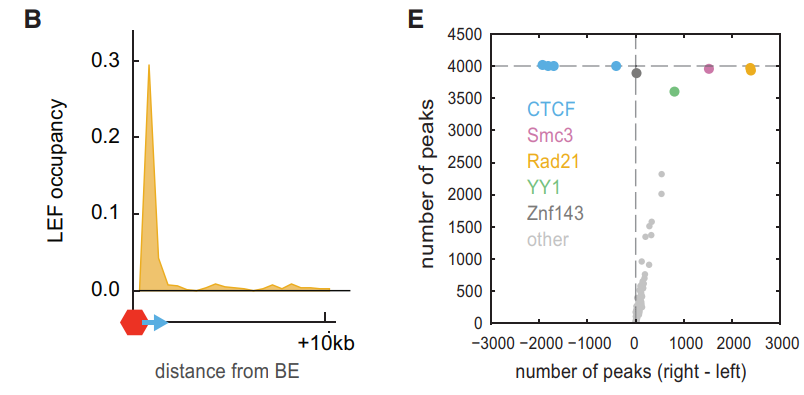
\includegraphics[width=0.8\textwidth]{assets/Snipaste_2023-01-13_19-41-04.png}
  \caption{\textbf{The Orientation Dependent Accumulation of Cohesin.} This figure is part of Figure 6 in \cite{fudenberg_formation_2016}. Fig B shows the theoretical explanation of the orientation-dependent enrichment of cohesin. Fig E shows the experimental data of cohesin ChIP-seq peaks at strong CTCF binding sites.}
  \label{fig:Exploration of Boundary Elements Properties}
\end{figure}

Furthermore, with the model at hand, the authors modify the BE permeability and directionality to try to recapitulate the effect of CTCF on TAD boundary. To correctly model and reproduce the experimental data, the authors converted ChIP-seq data for CTCF into BE permeability and directionality parameters with the help of cohesin peak and logistic transformation. According to the simulation and the analysis by the authors, the model to some extent reproduce and predicts the effect of CTCF on TAD boundary, yet agreement along the chromosome was non-uniform. However, the results do reflect that the increased permeability of BEs can lead to the emergence of large, homogeneous TADs, suggesting the importance of BEs in the formation of TADs and further supporting the model.

% insert figure 9
\begin{figure}[htbp]
  \centering
  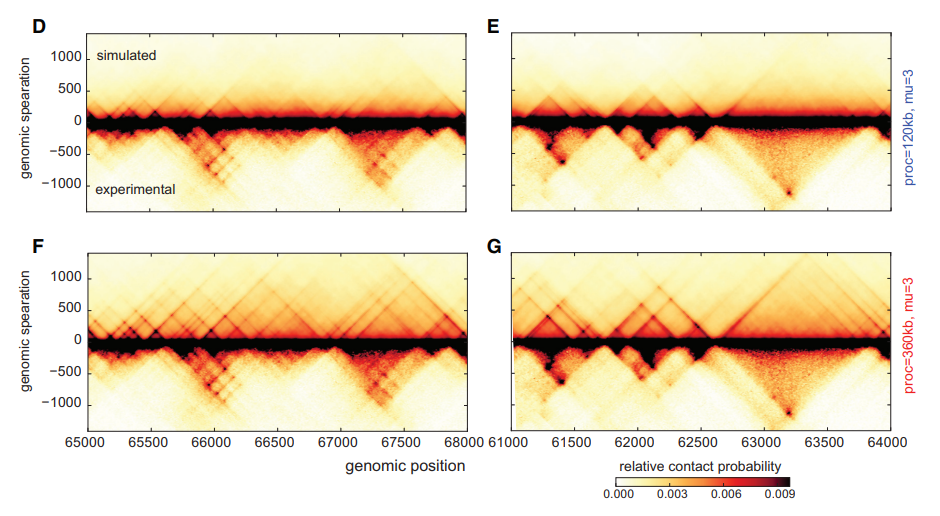
\includegraphics[width=0.8\textwidth]{assets/Snipaste_2023-01-13_19-45-50.png}
  \caption{\textbf{Simulation of Changing TAD Boundaries with Different BE Permeability. } This figure is part of Figure 7 in \cite{fudenberg_formation_2016}. LEF processivity is 120 kb (D and E) and 360 kb (F and G).}
  \label{fig:Simulation of Changing TAD Boundaries with Different BE Permeability}
\end{figure}

\section{Strengths and Weaknesses of the Paper}

\subsection*{Strengths}

The paper proposed and examined a model for an important 3D chromosomal structure and showed that the model is capable of reproducing the formation of TADs in the simulation. The model is also capable of predicting the effect of BEs on TADs, which is a very important step towards understanding the mechanism of TAD formation.

To the best of my knowledge, this is the first paper that proposed a model for TAD formation with detailed and rigorous simulation as well as predictive power. The model is also very simple and easy to understand, which makes it a very good starting point for further research on TAD formation.

\subsection*{Weaknesses}

Since this is one of the pioneering work, parts of the model still needs refinement and describe. For example, it is likely that the association possibility and dissociation possibility are not homogeneous across the genome. The ChIP-seq data of CTCF enrichment peaks were also not well modelled and reproduced in the simulation.

\section{Future Prospectives}

As is mentioned in the weaknesses, the models can be further refined to incorporate more subtleness in the chromatin conformational change. But the most important future work is to test the model in real biological systems, such as testing the proposed molecular candidate of BEs and LEFs. And in a paper published in 2019 \cite{kim_human_2019}, the loop extruding effect of cohesin has been proved, strongly supporting the model proposed in this paper.

% Bibliography
\printbibliography

\end{document}
